\documentclass[10pt,a4paper]{article}

% -----------------------------------------------------------------------------
% MATHS MANTHAN | Class 10 Circles Handbook | Academic Year 2026--27
% Publication-Quality Formula & Concept Master Handbook for CBSE Class 10
% Fully compliant with rationalized CBSE 2026--27 curriculum (Chapter 10: Circles)
% Compile with pdfLaTeX twice to resolve LastPage and cross-references.
% -----------------------------------------------------------------------------

\usepackage[a4paper,top=12mm,bottom=16mm,left=15mm,right=15mm,footskip=8mm]{geometry}
\usepackage[T1]{fontenc}
\usepackage{lmodern}
\usepackage{microtype}
\usepackage{amsmath,amssymb}
\usepackage[table]{xcolor}
\usepackage{array,tabularx,booktabs}
\usepackage{graphicx}
\usepackage{eso-pic}
\usepackage{tikz}
\usetikzlibrary{calc,positioning,arrows.meta,shapes.geometric,patterns}
\usepackage[most]{tcolorbox}
\usepackage{enumitem}
\usepackage{fancyhdr}
\usepackage{lastpage}
\usepackage[hidelinks]{hyperref}
\usepackage{url}

% Compatibility fix for colortbl + tabularx p-column alignment
\makeatletter
\let\insert@pcolumn\insert@column
\makeatother

% ============================================================================
% BRAND COLOR PALETTE — 100% UNIFORM WITH MATHS MANTHAN STANDARDS
% Primary Navy: #001F49 | Brand Gold: #D19029 | Secondary Slate: #4B5563
% ============================================================================
\definecolor{primary}{RGB}{0,31,73}
\definecolor{brandnavy}{RGB}{0,31,73}
\definecolor{accent}{RGB}{209,144,41}
\definecolor{brandgold}{RGB}{209,144,41}
\definecolor{secondary}{RGB}{75,85,99}
\definecolor{lightgray}{RGB}{246,248,250}
\definecolor{accentlight}{RGB}{254,250,242}
\definecolor{primarylight}{RGB}{240,244,250}

\colorlet{navy}{primary}
\colorlet{blue}{primary!82!black}
\colorlet{gold}{accent}
\colorlet{goldpale}{accentlight}
\colorlet{bluepale}{primarylight}
\colorlet{ink}{secondary}
\colorlet{muted}{secondary}
\colorlet{linegray}{primary!25}
\colorlet{reddeep}{primary}
\colorlet{redpale}{lightgray}
\colorlet{green}{primary}
\colorlet{greenpale}{primarylight}

% Automatic low-opacity logo watermark on every page
\IfFileExists{mathsmanthan logo.png}{%
  \AddToShipoutPictureBG{%
    \begin{tikzpicture}[remember picture,overlay]
      \node[opacity=0.065] at (current page.center) {%
        \includegraphics[width=0.55\paperwidth,keepaspectratio]{mathsmanthan logo.png}%
      };
    \end{tikzpicture}%
  }%
}{}

\hypersetup{
  pdftitle={Class 10 Circles | Maths Manthan Master Handbook},
  pdfauthor={Maths Manthan Tuition Classes},
  pdfsubject={CBSE Class 10 Mathematics, Academic Year 2026--27},
  pdfkeywords={Circles, Tangents, Class 10, CBSE, Geometry, Maths Manthan, Formula Handbook, 2026-27}
}

\setlength{\parindent}{0pt}
\setlength{\parskip}{2.5pt}
\renewcommand{\arraystretch}{1.15}
\setlist[itemize]{leftmargin=5mm,itemsep=1.5pt,topsep=1.5pt,parsep=0pt}
\setlist[enumerate]{leftmargin=5.5mm,itemsep=1.5pt,topsep=1.5pt,parsep=0pt}
\setlength{\tabcolsep}{4.5pt}
\emergencystretch=2em
\hfuzz=1pt

% ============================================================================
% HEADER / FOOTER SPECIFICATION
% ============================================================================
\newcommand{\TuitionName}{{\color{primary}MATHS} {\color{accent}MANTHAN}}
\newcommand{\TuitionSub}{{\color{primary}\textbullet\ \ \text{TUITION CLASSES}\ \ \textbullet}}
\newcommand{\ContactInfo}{e-mail: contact@mathsmanthan.co.in \quad$\vert$\quad Helpline: +91-8171546558}
\newcommand{\HandbookFooterTitle}{Class 10 Circles Handbook}

\pagestyle{fancy}
\fancyhf{}
\renewcommand{\headrulewidth}{0pt}
\renewcommand{\footrulewidth}{0.6pt}
\renewcommand{\footrule}{\hbox to\headwidth{\color{primary!30}\leaders\hrule height 0.6pt\hfill}}
\fancyfoot[L]{\footnotesize\href{https://mathsmanthan.co.in}{\textcolor{secondary}{\TuitionName\ $\vert$\ \HandbookFooterTitle}}}
\fancyfoot[R]{\footnotesize\textbf{\color{primary}Page \thepage\ of \pageref{LastPage}}\quad\textcolor{accent}{\textbf{Academic Year 2026--27}}}

\fancypagestyle{plain}{%
  \fancyhf{}
  \fancyfoot[L]{\footnotesize\href{https://mathsmanthan.co.in}{\textcolor{secondary}{\TuitionName\ $\vert$\ \HandbookFooterTitle}}}
  \fancyfoot[R]{\footnotesize\textbf{\color{primary}Page \thepage\ of \pageref{LastPage}}\quad\textcolor{accent}{\textbf{Academic Year 2026--27}}}
  \renewcommand{\headrulewidth}{0pt}
  \renewcommand{\footrulewidth}{0.6pt}
  \renewcommand{\footrule}{\hbox to\headwidth{\color{primary!30}\leaders\hrule height 0.6pt\hfill}}
}

% Institutional Brand Mark with TikZ Badge fallback
\newcommand{\BrandMark}{%
  \IfFileExists{mathsmanthan logo.png}{%
    \includegraphics[width=22mm,height=22mm,keepaspectratio]{mathsmanthan logo.png}%
  }{%
    
\begin{tikzpicture}[baseline=-0.6ex]
      \fill[navy,rounded corners=2.2pt] (0,0) rectangle (1.45,1.05);
      \draw[gold,line width=1.2pt] (0.15,0.15)--(1.30,0.15);
      \node[text=white,font=\sffamily\bfseries\Large] at (0.725,0.59) {MM};
    \end{tikzpicture}%
  }%
}

% Standard Chapter Banner
\newcommand{\chapterbanner}[4]{%
  \begin{tcolorbox}[enhanced,colback=bluepale,colframe=bluepale,boxrule=0pt,arc=2mm,
    left=3.5mm,right=3.5mm,top=2mm,bottom=2mm]
    {\footnotesize\bfseries\color{gold}CHAPTER #1\hfill\color{blue}#4}\par\vspace{0.6mm}
    {\LARGE\bfseries\color{navy}#2}\par
    {\small\color{muted}#3}
  \end{tcolorbox}\vspace{0.5mm}
}

% Standard Section Subhead
\newcommand{\subhead}[1]{%
  \vspace{1mm}{\large\bfseries\color{navy}#1}\par\vspace{0.4mm}
  {\color{gold}\rule{13mm}{1.2pt}}\par\vspace{0.8mm}
}

% Standard Color Boxes
\newtcolorbox{formulaBox}[1][]{enhanced,breakable,colback=goldpale,colframe=gold!65!black,
  boxrule=0.5pt,arc=1.5mm,left=3mm,right=3mm,top=1.8mm,bottom=1.8mm,
  before skip=2.5pt,after skip=3pt,#1}
\newtcolorbox{conceptBox}[1][]{enhanced,breakable,colback=bluepale,colframe=blue!25,
  boxrule=0.4pt,arc=1.5mm,left=3mm,right=3mm,top=1.8mm,bottom=1.8mm,
  before skip=2.5pt,after skip=3pt,#1}
\newtcolorbox{warningBox}[1][]{enhanced,breakable,colback=redpale,colframe=reddeep!45,
  boxrule=0.45pt,arc=1.5mm,left=3mm,right=3mm,top=1.8mm,bottom=1.8mm,
  before skip=2.5pt,after skip=3pt,#1}
\newtcolorbox{successBox}[1][]{enhanced,breakable,colback=greenpale,colframe=green!35,
  boxrule=0.45pt,arc=1.5mm,left=3mm,right=3mm,top=1.8mm,bottom=1.8mm,
  before skip=2.5pt,after skip=3pt,#1}

% Semantic Badges / Tags
\newcommand{\CoreTag}{\tcbox[colback=greenpale,colframe=green!40,boxrule=.3pt,arc=1mm,left=1.5mm,right=1.5mm,top=.4mm,bottom=.4mm]{\scriptsize\bfseries\color{green}CORE SYLLABUS}}
\newcommand{\ExamTag}{\tcbox[colback=bluepale,colframe=blue!25,boxrule=.3pt,arc=1mm,left=1.5mm,right=1.5mm,top=.4mm,bottom=.4mm]{\scriptsize\bfseries\color{blue}EXAM STRATEGY}}
\newcommand{\TrapTag}{\tcbox[colback=redpale,colframe=reddeep!40,boxrule=.3pt,arc=1mm,left=1.5mm,right=1.5mm,top=.4mm,bottom=.4mm]{\scriptsize\bfseries\color{reddeep}TRAP ALERT}}
\newcommand{\WorkedTag}{\tcbox[colback=bluepale,colframe=blue!25,boxrule=.3pt,arc=1mm,left=1.5mm,right=1.5mm,top=.4mm,bottom=.4mm]{\scriptsize\bfseries\color{blue}WORKED MODEL}}
\newcommand{\SupportTag}{\tcbox[colback=accentlight,colframe=gold!55!black,boxrule=.3pt,arc=1mm,left=1.5mm,right=1.5mm,top=.4mm,bottom=.4mm]{\scriptsize\bfseries\color{primary}SUPPORTING SKILL}}
\newcommand{\ReferenceTag}{\tcbox[colback=bluepale,colframe=blue!25,boxrule=.3pt,arc=1mm,left=1.5mm,right=1.5mm,top=.4mm,bottom=.4mm]{\scriptsize\bfseries\color{primary}REFERENCE MATRIX}}
\newcommand{\ExtensionTag}{\tcbox[colback=goldpale,colframe=gold!55,boxrule=.3pt,arc=1mm,left=1.5mm,right=1.5mm,top=.4mm,bottom=.4mm]{\scriptsize\bfseries\color{gold!50!black}EXTENSION PRACTICE}}

\begin{document}

% =============================================================================
% PAGE 1: STANDALONE INSTITUTIONAL COVER PAGE
% =============================================================================
\thispagestyle{fancy}
\vspace*{0mm}

\noindent
\makebox[0pt][l]{%
  \raisebox{-0.80cm}[0pt][0pt]{%
    \href{https://mathsmanthan.co.in}{\BrandMark}%
  }%
}%
\parbox{\textwidth}{%
  \centering
  \href{https://mathsmanthan.co.in}{%
    {\fontsize{23pt}{23pt}\selectfont\bfseries \TuitionName}\\[3pt]
    {\footnotesize\bfseries \TuitionSub}%
  }\\[2pt]
  {\scriptsize\color{secondary} \ContactInfo}
}

\vspace{5pt}
\noindent{\color{primary}\rule{0.72\textwidth}{1.5pt}}\hfill{\color{accent}\rule{0.26\textwidth}{1.5pt}}

\vspace{4mm}
\begin{center}
  {\large\bfseries\color{muted}CBSE CLASS 10 \;|\; MATHEMATICS}\\[3.5mm]
  {\fontsize{28}{33}\selectfont\bfseries\color{navy}CIRCLES}\\[2mm]
  {\Large\color{blue}Master Concept, Formula \& Visual Problem-Solving Handbook}\\[2.5mm]
  {\large\color{gold}\bfseries Academic Year 2026--27}
\end{center}

\vspace{3mm}
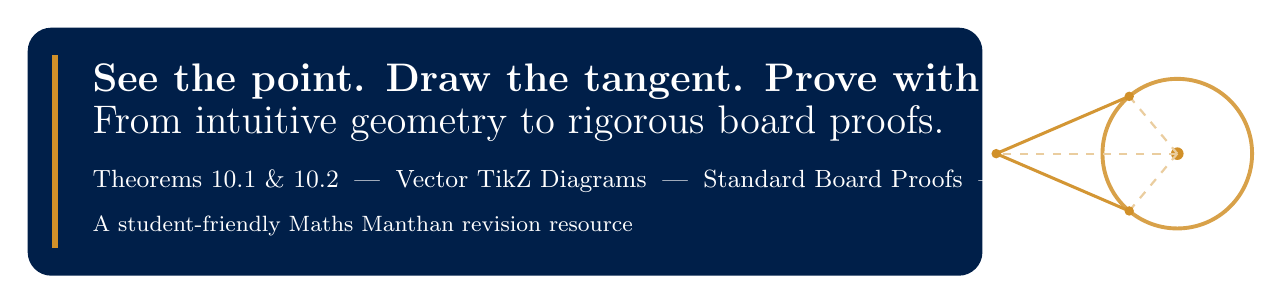
\begin{tikzpicture}
  \fill[navy,rounded corners=3mm] (0,0) rectangle (\textwidth,3.15);
  \draw[gold,line width=2pt] (0.35,0.35)--(0.35,2.80);
  \node[anchor=west,text=white,font=\bfseries\Large] at (0.7,2.46) {See the point. Draw the tangent. Prove with confidence.};
  \node[anchor=west,text=white,font=\Large] at (0.7,1.93) {From intuitive geometry to rigorous board proofs.};
  \node[anchor=west,text=white,font=\small] at (0.7,1.20) {Theorems 10.1 \& 10.2 \;|\; Vector TikZ Diagrams \;|\; Standard Board Proofs \;|\; Exam Traps};
  \node[anchor=west,text=white!75,font=\footnotesize] at (0.7,0.63) {A student-friendly Maths Manthan revision resource};
  
  % Geometric Circle and Tangent motif in gold
  \coordinate (C) at (14.6, 1.55);
  \draw[gold!85, line width=1.4pt] (C) circle (0.95);
  \fill[gold] (C) circle (0.08);
  \coordinate (T1) at ($(C)+(130:0.95)$);
  \coordinate (T2) at ($(C)+(230:0.95)$);
  \coordinate (Pext) at (12.3, 1.55);
  \draw[gold!95, line width=1.1pt] (Pext) -- (T1);
  \draw[gold!95, line width=1.1pt] (Pext) -- (T2);
  \draw[gold!45, line width=0.8pt, dashed] (C) -- (T1);
  \draw[gold!45, line width=0.8pt, dashed] (C) -- (T2);
  \draw[gold!45, line width=0.8pt, dashed] (C) -- (Pext);
  \fill[gold] (T1) circle (0.06);
  \fill[gold] (T2) circle (0.06);
  \fill[gold] (Pext) circle (0.06);
\end{tikzpicture}

\vspace{3.5mm}
\begin{minipage}[t]{0.48\textwidth}
  \begin{conceptBox}[title=What this handbook includes,fonttitle=\bfseries\color{navy}]
    \begin{itemize}
      \item Complete definitions: Secant vs. Tangent \& Point of Contact.
      \item Rigorous proofs of \textbf{Theorem 10.1} (Radius $\perp$ Tangent) and \textbf{Theorem 10.2} (Equal Tangents).
      \item Right-triangle Pythagorean models \& angle relationships.
      \item Circumscribed polygon master results ($AB+CD=BC+DA$).
      \item Concentric circle chords and incircle radius formulas.
    \end{itemize}
  \end{conceptBox}
\end{minipage}\hfill
\begin{minipage}[t]{0.48\textwidth}
  \begin{formulaBox}[title=How to use this handbook,fonttitle=\bfseries\color{navy}]
    \raggedright Always mark the radius to the point of contact first to expose the $90^\circ$ angle. Identify whether the problem relies on \textbf{Pythagoras} (length calculations) or \textbf{cyclic properties / isosceles triangles} (angle determinations). Write full geometric reasons in board exam answers.
  \end{formulaBox}
\end{minipage}

\vspace{1.5mm}
\begin{warningBox}[title=Official CBSE Curriculum Scope (Academic Year 2026--27),fonttitle=\bfseries\color{navy}]
  \textbf{Zero Deleted Content in Chapter 10:} The rationalized NCERT Class 10 curriculum retains Chapter 10: \textit{Circles} in its entirety under Unit IV: Geometry. Both core theorems and their applications are strictly tested. Note: Geometric constructions of tangents (formerly Chapter 11) remain \textbf{permanently excluded} from the syllabus. Chord theorems and cyclic quadrilaterals belong to Class 9 and serve solely as background tools.
  {\scriptsize Source: \href{https://cbseacademic.nic.in/web_material/CurriculumMain27/SecPart1/Maths_SecP1X_2026-27.pdf}{CBSE Secondary Curriculum (2026--27), Unit IV: Geometry}.}
\end{warningBox}

\vfill
\begin{center}
  {\small\bfseries\color{navy}Maths Manthan Tuition Classes}\\
  {\footnotesize\color{muted}contact@mathsmanthan.co.in \quad\textbar\quad +91-8171546558}\\
  {\footnotesize\url{https://mathsmanthan.co.in}}\\[2.5mm]
  {\scriptsize\color{muted}Prepared for learning and revision \;--\; not an official CBSE publication.}
\end{center}

\clearpage

% =============================================================================
% PAGE 2: MODULE 1 — FOUNDATIONAL GEOMETRY OF CIRCLES (PREREQUISITES)
% =============================================================================
\thispagestyle{fancy}
\vspace*{0mm}

\chapterbanner{10}{FOUNDATIONAL GEOMETRY OF CIRCLES}{Radius, Diameter, Chord, Secant, and Tangent -- The Vocabulary of Circles}{\SupportTag}

\subhead{Module 1.1 $\vert$ The Circle as a Geometric Locus}
A \textbf{circle} is the collection of all points in a plane equidistant from a fixed point (centre $O$).
\begin{itemize}
  \item \textbf{Centre ($O$):} Fixed point. \quad \textbf{Radius ($r$):} Fixed distance from centre to boundary ($r > 0$).
  \item \textbf{Three Regions:} Interior ($OP < r$), On the circle ($OP = r$), and Exterior ($OP > r$).
\end{itemize}

\subhead{Module 1.2 $\vert$ Anatomy of Line Segments Associated with a Circle}

\begin{center}
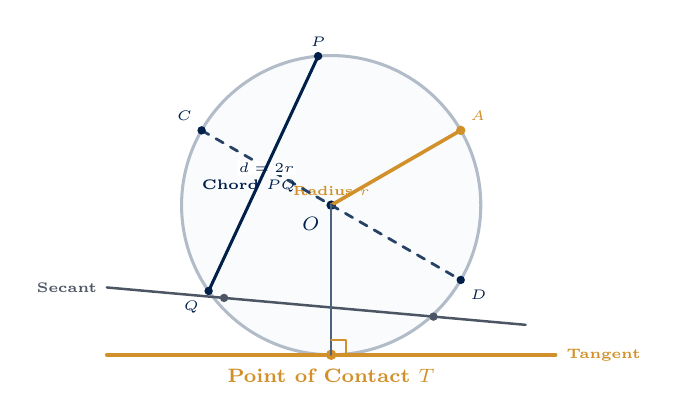
\begin{tikzpicture}[scale=0.95, line cap=round, line join=round]
  \coordinate (O) at (0,0);
  \def\R{2.0}
  \draw[primary!30, fill=primarylight!40, line width=1.1pt] (O) circle (\R);
  \fill[primary] (O) circle (1.8pt) node[below left=1pt, font=\scriptsize\bfseries\color{navy}]{$O$};
  
  % Radius OA
  \coordinate (A) at (30:\R);
  \draw[accent, line width=1.3pt] (O) -- (A);
  \fill[accent] (A) circle (1.8pt) node[above right, font=\tiny\bfseries\color{accent}]{$A$};
  \node[font=\tiny\bfseries\color{accent}, midway, above] at ($(O)!0.5!(A)$) {Radius $r$};

  % Diameter CD
  \coordinate (C) at (150:\R);
  \coordinate (D) at (-30:\R);
  \draw[navy!85, line width=1pt, dashed] (C) -- (D);
  \fill[navy] (C) circle (1.6pt) node[above left, font=\tiny\bfseries\color{navy}]{$C$};
  \fill[navy] (D) circle (1.6pt) node[below right, font=\tiny\bfseries\color{navy}]{$D$};
  \node[font=\tiny\bfseries\color{navy}, fill=white, inner sep=0.8pt] at ($(O)!0.5!(C)$) {$d=2r$};

  % Chord PQ
  \coordinate (Pchord) at (95:\R);
  \coordinate (Qchord) at (215:\R);
  \draw[primary, line width=1.1pt] (Pchord) -- (Qchord);
  \fill[primary] (Pchord) circle (1.6pt) node[above, font=\tiny\bfseries\color{navy}]{$P$};
  \fill[primary] (Qchord) circle (1.6pt) node[below left, font=\tiny\bfseries\color{navy}]{$Q$};
  \node[font=\tiny\bfseries\color{primary}] at (-1.1,0.25) {Chord $PQ$};

  % Secant Line EF
  \coordinate (E) at (-3.0, -1.1);
  \coordinate (F) at (2.6, -1.6);
  \draw[secondary, line width=0.9pt] (E) -- (F);
  \node[font=\tiny\bfseries\color{secondary}, left] at (E) {Secant};
  \fill[secondary] ($(E)!0.28!(F)$) circle (1.6pt);
  \fill[secondary] ($(E)!0.78!(F)$) circle (1.6pt);

  % Tangent Line at T (0, -\R)
  \coordinate (T) at (0,-\R);
  \draw[accent, line width=1.3pt] (-3.0,-\R) -- (3.0,-\R) node[right, font=\tiny\bfseries\color{accent}]{Tangent};
  \fill[accent] (T) circle (2pt) node[below=1.5pt, font=\scriptsize\bfseries\color{accent}]{Point of Contact $T$};
  \draw[primary!70, line width=0.9pt] (O) -- (T);
  \draw[accent, line width=0.7pt] (0.2,-\R) -- (0.2,-\R+0.2) -- (0,-\R+0.2);
\end{tikzpicture}
\end{center}

\vspace{-1mm}
\subhead{Module 1.3 $\vert$ Line-Circle Relationship Taxonomy}

Let $d$ be the perpendicular distance from centre $O$ to line $l$:

\begin{center}
\small
\begin{tabularx}{\textwidth}{>{\bfseries\color{navy}}p{28mm} c c X}
\toprule
\rowcolor{bluepale}Relationship & Condition & Common Points & Geometric Identity and Property \\
\midrule
Non-Intersecting & $d > r$ & $0$ & Line lies completely outside the circle. No intersection. \\
Secant & $d < r$ & $2$ & Line cuts the circle at two distinct points. Chord is internal segment. \\
Tangent & $d = r$ & $1$ & Line touches circle at \textbf{one unique point}. Limiting case of secant. \\
\bottomrule
\end{tabularx}
\end{center}

\begin{conceptBox}[title=Pedagogical Insight: Tangent as the Limiting Position of a Secant,fonttitle=\bfseries\color{navy}]
  Imagine secant $AB$ cutting the circle at $A$ and $B$. As secant line rotates such that chord length $AB \to 0$, points $A$ and $B$ merge into a single coincident point. The secant smoothly transitions into a \textbf{tangent}. This provides the foundational intuition of tangent lines in calculus and geometry.
\end{conceptBox}

\clearpage

% =============================================================================
% PAGE 3: MODULE 2 — THE TANGENT TO A CIRCLE & NUMBER OF TANGENTS
% =============================================================================
\thispagestyle{fancy}
\vspace*{0mm}

\chapterbanner{10}{THE TANGENT TO A CIRCLE}{Definition, Point of Contact \& The Three Positional Cases}{\CoreTag}

\subhead{Module 2.1 $\vert$ Formal Definition of a Tangent}

\begin{formulaBox}
  A \textbf{tangent} to a circle is a straight line that touches the circle at \textbf{only one point}:
  \[
    l \cap C(O, r) = \{P\}
  \]
  The unique point $P$ common to the line and the circle is called the \textbf{Point of Contact} (or \textit{Point of Tangency}).
\end{formulaBox}

\subhead{Module 2.2 $\vert$ Geometric Comparison: Secant vs. Tangent}

\begin{center}
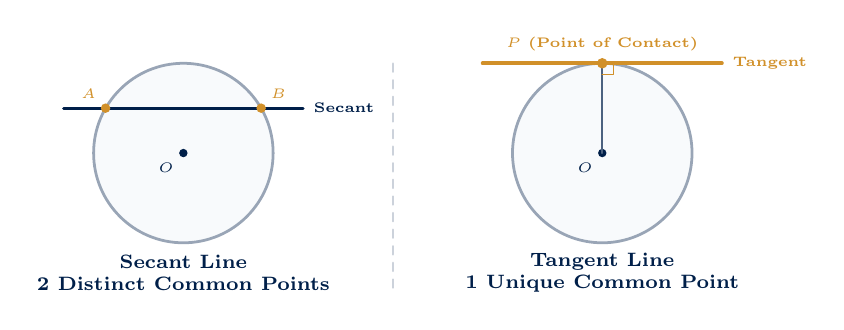
\begin{tikzpicture}[scale=0.95, line cap=round, line join=round]
  % Secant
  \begin{scope}[shift={(0,0)}]
    \coordinate (O1) at (0,0);
    \draw[navy!40, fill=bluepale!50, line width=1pt] (O1) circle (1.2);
    \fill[navy] (O1) circle (1.6pt) node[below left, font=\tiny\bfseries\color{navy}]{$O$};
    \draw[navy, line width=1.2pt] (-1.6, 0.6) -- (1.6, 0.6) node[right, font=\tiny\bfseries]{Secant};
    \fill[accent] (-1.04, 0.6) circle (1.8pt) node[above left, font=\tiny\bfseries\color{accent}]{$A$};
    \fill[accent] (1.04, 0.6) circle (1.8pt) node[above right, font=\tiny\bfseries\color{accent}]{$B$};
    \node[align=center, font=\scriptsize\bfseries\color{navy}] at (0,-1.6) {\textbf{Secant Line}\\2 Distinct Common Points};
  \end{scope}

  \draw[primary!20, line width=0.8pt, dashed] (2.8,-1.8) -- (2.8,1.2);

  % Tangent
  \begin{scope}[shift={(5.6,0)}]
    \coordinate (O2) at (0,0);
    \draw[navy!40, fill=bluepale!50, line width=1pt] (O2) circle (1.2);
    \fill[navy] (O2) circle (1.6pt) node[below left, font=\tiny\bfseries\color{navy}]{$O$};
    \draw[accent, line width=1.3pt] (-1.6, 1.2) -- (1.6, 1.2) node[right, font=\tiny\bfseries\color{accent}]{Tangent};
    \draw[navy!70, line width=0.8pt] (O2) -- (0, 1.2);
    \fill[accent] (0, 1.2) circle (2pt) node[above=1pt, font=\tiny\bfseries\color{accent}]{$P$ (Point of Contact)};
    \draw[accent, line width=0.6pt] (0.15,1.2) -- (0.15,1.05) -- (0,1.05);
    \node[align=center, font=\scriptsize\bfseries\color{navy}] at (0,-1.6) {\textbf{Tangent Line}\\1 Unique Common Point};
  \end{scope}
\end{tikzpicture}
\end{center}

\vspace{-1mm}
\subhead{Module 2.3 $\vert$ Number of Tangents from a Point to a Circle (The 3 Positional Cases)}

\begin{center}
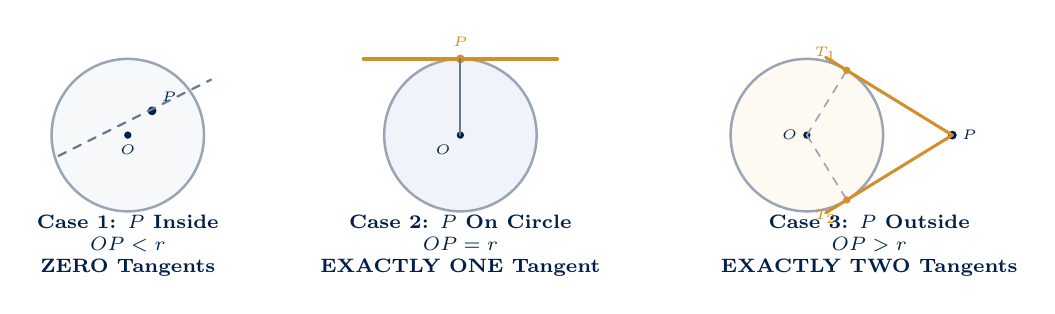
\begin{tikzpicture}[scale=0.88, line cap=round, line join=round]
  % Case 1: Point Inside
  \begin{scope}[shift={(0,0)}]
    \coordinate (O) at (0,0);
    \draw[primary!40, fill=lightgray, line width=0.9pt] (O) circle (1.1);
    \fill[primary] (O) circle (1.5pt) node[below, font=\tiny\bfseries]{$O$};
    \fill[reddeep] (0.35, 0.35) circle (1.8pt) node[above right, font=\tiny\bfseries\color{reddeep}]{$P$};
    \draw[reddeep!60, line width=0.8pt, dashed] (-1.0,-0.3) -- (1.2,0.8);
    \node[font=\scriptsize\bfseries\color{navy}, align=center] at (0,-1.6) {\textbf{Case 1: $P$ Inside}\\$OP < r$\\\textbf{ZERO Tangents}};
  \end{scope}

  % Case 2: Point On
  \begin{scope}[shift={(4.8,0)}]
    \coordinate (O) at (0,0);
    \draw[primary!40, fill=bluepale, line width=0.9pt] (O) circle (1.1);
    \fill[primary] (O) circle (1.5pt) node[below left, font=\tiny\bfseries]{$O$};
    \fill[accent] (0, 1.1) circle (1.8pt) node[above=1pt, font=\tiny\bfseries\color{accent}]{$P$};
    \draw[accent, line width=1.2pt] (-1.4,1.1) -- (1.4,1.1);
    \draw[primary!60, line width=0.7pt] (O) -- (0, 1.1);
    \node[font=\scriptsize\bfseries\color{navy}, align=center] at (0,-1.6) {\textbf{Case 2: $P$ On Circle}\\$OP = r$\\\textbf{EXACTLY ONE Tangent}};
  \end{scope}

  % Case 3: Point Outside
  \begin{scope}[shift={(9.8,0)}]
    \coordinate (O) at (0,0);
    \draw[primary!40, fill=accentlight, line width=0.9pt] (O) circle (1.1);
    \fill[primary] (O) circle (1.5pt) node[left, font=\tiny\bfseries]{$O$};
    \coordinate (P) at (2.1, 0);
    \fill[primary] (P) circle (1.8pt) node[right, font=\tiny\bfseries\color{primary}]{$P$};
    \coordinate (T1) at (0.576, 0.936);
    \coordinate (T2) at (0.576, -0.936);
    \draw[accent, line width=1.1pt] (P) -- ($(P)!1.2!(T1)$);
    \draw[accent, line width=1.1pt] (P) -- ($(P)!1.2!(T2)$);
    \draw[primary!40, dashed, line width=0.6pt] (O) -- (T1);
    \draw[primary!40, dashed, line width=0.6pt] (O) -- (T2);
    \fill[accent] (T1) circle (1.5pt) node[above left, font=\tiny\bfseries]{$T_1$};
    \fill[accent] (T2) circle (1.5pt) node[below left, font=\tiny\bfseries]{$T_2$};
    \node[font=\scriptsize\bfseries\color{navy}, align=center] at (0.9,-1.6) {\textbf{Case 3: $P$ Outside}\\$OP > r$\\\textbf{EXACTLY TWO Tangents}};
  \end{scope}
\end{tikzpicture}
\end{center}

\vspace{-1mm}
\begin{warningBox}[title=Board Exam Objective Trap: Tangent Counts,fonttitle=\bfseries\color{reddeep}]
  \begin{itemize}
    \item "Tangents through a point \textbf{lying on} the circle?" $\longrightarrow$ \textbf{1}.
    \item "Tangents \textbf{from an external point}?" $\longrightarrow$ \textbf{2}.
    \item "Maximum number of parallel tangents to a circle?" $\longrightarrow$ \textbf{2} (at opposite ends of a diameter).
    \item "Total number of tangents that can be drawn to a circle?" $\longrightarrow$ \textbf{Infinitely many}.
  \end{itemize}
\end{warningBox}

\clearpage

% =============================================================================
% PAGE 4: MODULE 3 — THEOREM 10.1 (TANGENT IS PERPENDICULAR TO RADIUS)
% =============================================================================
\thispagestyle{fancy}
\vspace*{0mm}

\chapterbanner{10}{THEOREM 10.1: RADIUS $\perp$ TANGENT}{The Fundamental Orthogonality Property at the Point of Contact}{\CoreTag}

\subhead{Module 3.1 $\vert$ Official Theorem Statement}

\begin{formulaBox}
  \textbf{CBSE Theorem 10.1:} \\
  \textit{The tangent at any point of a circle is perpendicular to the radius through the point of contact.}
  \[
    \boxed{OP \perp XY \quad \iff \quad \angle OPX = \angle OPY = 90^\circ}
  \]
  where $O$ is the centre, $P$ is the point of contact, and $XY$ is the tangent line.
\end{formulaBox}

\subhead{Module 3.2 $\vert$ Standard CBSE Board Proof (Shortest Distance Property)}

\begin{minipage}[t]{0.54\textwidth}
  \textbf{Given:} A circle $C(O, r)$ and a tangent $XY$ touching at $P$.\\
  \textbf{To Prove:} $OP \perp XY$.\\
  \textbf{Construction:} Take any point $Q$ on $XY$ ($Q \neq P$). Join $OQ$, intersecting the circle at point $R$.
  
  \vspace{1mm}
  \textbf{Proof Steps:}
  \begin{enumerate}[leftmargin=4.5mm, itemsep=1.5pt]
    \item Point $Q$ must lie \textbf{outside} the circle. (If $Q$ were inside, $XY$ would be a secant, not a tangent).
    \item Therefore, $OQ > OR$.
    \item But $OR = OP$ (radii of the same circle).
    \item Hence, $OQ > OP$ for every point $Q \in XY$ ($Q \neq P$).
    \item Thus, $OP$ is the \textbf{shortest distance} from centre $O$ to any point on line $XY$.
    \item Since the shortest distance from a point to a line is the perpendicular distance:
      \[
        \mathbf{OP \perp XY}. \quad \text{\textbf{[Q.E.D.]}}
      \]
  \end{enumerate}
\end{minipage}\hfill
\begin{minipage}[t]{0.43\textwidth}
  \begin{center}
  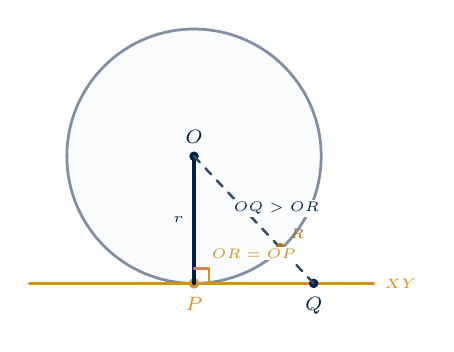
\begin{tikzpicture}[scale=0.95, line cap=round, line join=round]
    \coordinate (O) at (0,1.7);
    \def\r{1.7}
    \draw[navy!50, fill=bluepale!40, line width=1pt] (O) circle (\r);
    \fill[navy] (O) circle (1.8pt) node[above=1pt, font=\scriptsize\bfseries\color{navy}]{$O$};

    \coordinate (P) at (0,0);
    \draw[accent, line width=1.3pt] (-2.2,0) -- (2.4,0) node[right, font=\tiny\bfseries\color{accent}]{$XY$};
    \fill[accent] (P) circle (2pt) node[below=1.5pt, font=\scriptsize\bfseries\color{accent}]{$P$};

    \draw[primary, line width=1.2pt] (O) -- (P) node[midway, left, font=\tiny\bfseries]{$r$};
    \draw[accent, line width=0.8pt] (0.2,0) -- (0.2,0.2) -- (0,0.2);

    \coordinate (Q) at (1.6,0);
    \fill[reddeep] (Q) circle (1.8pt) node[below=1.5pt, font=\scriptsize\bfseries\color{reddeep}]{$Q$};
    \draw[navy!80, line width=0.9pt, dashed] (O) -- (Q);
    
    \coordinate (R) at ($(O)!0.72!(Q)$);
    \fill[gold!80!black] (R) circle (1.8pt) node[above right, font=\tiny\bfseries]{$R$};

    \node[font=\tiny\bfseries\color{navy}, fill=white, inner sep=0.8pt] at (1.1, 1.0) {$OQ > OR$};
    \node[font=\tiny\bfseries\color{accent}, fill=white, inner sep=0.8pt] at (0.8, 0.4) {$OR = OP$};
  \end{tikzpicture}
  \end{center}
\end{minipage}

\vspace{-1mm}
\subhead{Module 3.3 $\vert$ Vital Converse and Diameter Corollary}

\begin{conceptBox}[title=Converse of Theorem 10.1,fonttitle=\bfseries\color{navy}]
  \textit{A line drawn through the endpoint of a radius and perpendicular to it is a tangent to the circle.}
\end{conceptBox}

\begin{successBox}[title=Core Board Corollary: Parallel Tangents at Diameter Ends,fonttitle=\bfseries\color{green}]
  The tangents drawn at the ends of any diameter of a circle are \textbf{parallel}.
  \begin{itemize}
    \item Let $AB$ be a diameter. Tangent $l_1$ at $A$ has $\angle OAX = 90^\circ$; tangent $l_2$ at $B$ has $\angle OBY = 90^\circ$.
    \item Since interior alternate angles are equal ($\angle OAX = \angle OBY = 90^\circ$), $l_1 \parallel l_2$.
    \item \textbf{Board Rule:} A circle can have at most \textbf{two parallel tangents} along any direction.
  \end{itemize}
\end{successBox}

\clearpage

% =============================================================================
% PAGE 5: MODULE 4 — THEOREM 10.2 (TANGENTS FROM AN EXTERNAL POINT)
% =============================================================================
\thispagestyle{fancy}
\vspace*{0mm}

\chapterbanner{10}{THEOREM 10.2: EQUALITY OF TANGENT LENGTHS}{RHS Congruence Proof, Angle Bisectors \& Line of Centres}{\CoreTag}

\subhead{Module 4.1 $\vert$ Official Theorem Statement}

\begin{formulaBox}
  \textbf{CBSE Theorem 10.2:} \\
  \textit{The lengths of tangents drawn from an external point to a circle are equal.}
  \[
    \boxed{PA = PB}
  \]
  where $P$ is an external point, and $A$ and $B$ are the points of contact of the two tangents.
\end{formulaBox}

\subhead{Module 4.2 $\vert$ Standard CBSE Board Proof (RHS Congruence Model)}

\begin{minipage}[t]{0.54\textwidth}
  \textbf{Given:} A circle $C(O, r)$ and external point $P$. Tangents $PA$ and $PB$ touch at $A$ and $B$.\\
  \textbf{To Prove:} $PA = PB$.\\
  \textbf{Construction:} Join $OA, OB$, and $OP$.

  \vspace{1mm}
  \textbf{Proof Steps:}
  \begin{enumerate}[leftmargin=4.5mm, itemsep=2pt]
    \item In $\triangle OAP$ and $\triangle OBP$:
    \item $\angle OAP = \angle OBP = 90^\circ$ \\
      \textit{(Theorem 10.1: Radius $\perp$ Tangent at contact)}.
    \item $OP = OP$ \quad \textit{(Common hypotenuse)}.
    \item $OA = OB = r$ \quad \textit{(Radii of the same circle)}.
    \item Therefore, by \textbf{RHS Congruence Criterion}:
      \[
        \mathbf{\triangle OAP \cong \triangle OBP}
      \]
    \item By Corresponding Parts of Congruent Triangles (CPCTC):
      \[
        \mathbf{PA = PB}. \quad \text{\textbf{[Hence Proved]}}
      \]
  \end{enumerate}
\end{minipage}\hfill
\begin{minipage}[t]{0.43\textwidth}
  \begin{center}
  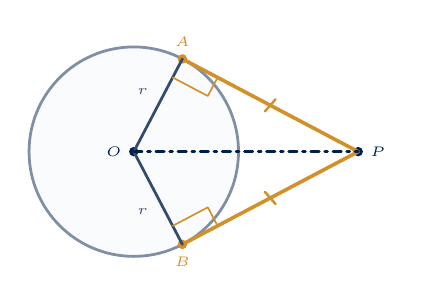
\begin{tikzpicture}[scale=0.95, line cap=round, line join=round]
    \coordinate (O) at (0,0);
    \def\r{1.4}
    \def\d{3.0}
    \coordinate (P) at (\d, 0);
    
    % Angle approx 62.2 degrees
    \coordinate (A) at (0.65, 1.24);
    \coordinate (B) at (0.65, -1.24);

    \draw[navy!50, fill=bluepale!35, line width=1pt] (O) circle (\r);
    \fill[navy] (O) circle (1.8pt) node[left=1pt, font=\tiny\bfseries\color{navy}]{$O$};
    \fill[primary] (P) circle (1.8pt) node[right=1pt, font=\tiny\bfseries\color{primary}]{$P$};

    \draw[accent, line width=1.3pt] (P) -- (A);
    \draw[accent, line width=1.3pt] (P) -- (B);
    \fill[accent] (A) circle (1.8pt) node[above=1pt, font=\tiny\bfseries\color{accent}]{$A$};
    \fill[accent] (B) circle (1.8pt) node[below=1pt, font=\tiny\bfseries\color{accent}]{$B$};

    \draw[primary!80, line width=1pt] (O) -- (A) node[midway, above left, font=\tiny\bfseries]{$r$};
    \draw[primary!80, line width=1pt] (O) -- (B) node[midway, below left, font=\tiny\bfseries]{$r$};
    \draw[navy, line width=1pt, dashdotted] (O) -- (P);

    % Right angles
    \draw[accent, line width=0.6pt] ($(A)!0.2!(P)$) -- ($(A)!0.2!(P) + (A)!0.2!(O) - (A)$) -- ($(A)!0.2!(O)$);
    \draw[accent, line width=0.6pt] ($(B)!0.2!(P)$) -- ($(B)!0.2!(P) + (B)!0.2!(O) - (B)$) -- ($(B)!0.2!(O)$);

    % Ticks on PA and PB
    \draw[accent, line width=0.9pt] ($(P)!0.5!(A) + (-0.07,-0.08)$) -- ($(P)!0.5!(A) + (0.07,0.08)$);
    \draw[accent, line width=0.9pt] ($(P)!0.5!(B) + (-0.07,0.08)$) -- ($(P)!0.5!(B) + (0.07,-0.08)$);
  \end{tikzpicture}
  \end{center}
\end{minipage}

\vspace{-1mm}
\subhead{Module 4.3 $\vert$ Three Indispensable Corollaries (CPCTC Yields)}

Because $\triangle OAP \cong \triangle OBP$, three critical geometric relationships follow immediately:
\begin{enumerate}[label=\textbf{\color{navy}Corollary \arabic*:}, leftmargin=24mm, itemsep=2pt]
  \item \textbf{Equal Tangent Angles ($\angle OPA = \angle OPB$):}\\
    $OP$ is the \textbf{angle bisector} of the angle between the two tangents ($\angle APB$).
  \item \textbf{Equal Central Angles ($\angle AOP = \angle BOP$):}\\
    $OP$ is the \textbf{angle bisector} of the central angle subtended by the contacts ($\angle AOB$).
  \item \textbf{Perpendicular Bisector of Chord ($OP \perp AB$):}\\
    If chord $AB$ connects points of contact, $OP$ is the \textbf{perpendicular bisector} of chord $AB$.
\end{enumerate}

\begin{conceptBox}[title=Summary Box: Mirror Symmetry of Line of Centres ($OP$),fonttitle=\bfseries\color{navy}]
  \[
    \boxed{PA = PB \qquad \angle OPA = \angle OPB = \frac{1}{2}\angle APB \qquad \angle AOP = \angle BOP = \frac{1}{2}\angle AOB}
  \]
\end{conceptBox}

\clearpage

% =============================================================================
% PAGE 6: MODULE 5 — THE TANGENT-RADIUS RIGHT TRIANGLE & PYTHAGORAS MODELS
% =============================================================================
\thispagestyle{fancy}
\vspace*{0mm}

\chapterbanner{10}{THE TANGENT-RADIUS RIGHT TRIANGLE}{Pythagorean Triplet Mechanics \& Standard Length Calculations}{\WorkedTag}

\subhead{Module 5.1 $\vert$ The Fundamental Tangent-Radius Right Triangle}

Because Theorem 10.1 guarantees $\angle OTP = 90^\circ$, triangle $\triangle OTP$ is always a \textbf{right triangle} with hypotenuse $OP$:

\begin{center}
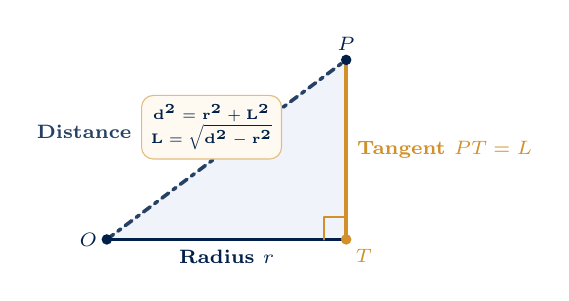
\begin{tikzpicture}[scale=0.95, line cap=round, line join=round]
  \coordinate (O) at (0,0);
  \coordinate (T) at (3.2,0);
  \coordinate (P) at (3.2,2.4);

  \fill[bluepale] (O) -- (T) -- (P) -- cycle;
  \draw[navy, line width=1.3pt] (O) -- (T) node[midway, below, font=\scriptsize\bfseries\color{navy}]{Radius $r$};
  \draw[accent, line width=1.3pt] (T) -- (P) node[midway, right, font=\scriptsize\bfseries\color{accent}]{Tangent $PT = L$};
  \draw[navy!85, line width=1.3pt, dashdotted] (O) -- (P) node[midway, above left, font=\scriptsize\bfseries\color{navy}]{Distance $OP = d$};

  \draw[accent, line width=0.8pt] (2.9,0) -- (2.9,0.3) -- (3.2,0.3);

  \fill[navy] (O) circle (2pt) node[left, font=\scriptsize\bfseries\color{navy}]{$O$};
  \fill[accent] (T) circle (2pt) node[below right, font=\scriptsize\bfseries\color{accent}]{$T$};
  \fill[primary] (P) circle (2pt) node[above, font=\scriptsize\bfseries\color{primary}]{$P$};

  \node[draw=gold!60, fill=goldpale, rounded corners=1.5mm, font=\tiny\bfseries\color{navy}, align=center] at (1.4,1.5) {
    $\mathbf{d^2 = r^2 + L^2}$\\
    $\mathbf{L = \sqrt{d^2 - r^2}}$
  };
\end{tikzpicture}
\end{center}

\vspace{-2mm}
\begin{formulaBox}
  \[
    \boxed{\text{Tangent Length } PT = \sqrt{OP^2 - r^2} \qquad \text{Radius } r = \sqrt{OP^2 - PT^2} \qquad \text{Distance } OP = \sqrt{PT^2 + r^2}}
  \]
\end{formulaBox}

\subhead{Module 5.2 $\vert$ Standard Pythagorean Triplets in Board Exams}
\begin{center}
\small
\begin{tabularx}{0.9\textwidth}{>{\bfseries\color{navy}}c c c >{\color{secondary}}X}
\toprule
\rowcolor{bluepale}Radius ($r$) & Tangent ($PT$) & Distance ($OP$) & Triplet Family \\
\midrule
$3\text{ cm}$ & $4\text{ cm}$ & $5\text{ cm}$ & $(3, 4, 5)$ or scaled $(6, 8, 10)$, $(9, 12, 15)$ \\
$5\text{ cm}$ & $12\text{ cm}$ & $13\text{ cm}$ & $(5, 12, 13)$ or scaled $(10, 24, 26)$ \\
$7\text{ cm}$ & $24\text{ cm}$ & $25\text{ cm}$ & $(7, 24, 25)$ \\
$8\text{ cm}$ & $15\text{ cm}$ & $17\text{ cm}$ & $(8, 15, 17)$ \\
\bottomrule
\end{tabularx}
\end{center}

\subhead{Module 5.3 $\vert$ Two Core Worked Archetypes}

\begin{conceptBox}[title=Worked Archetype 1: Calculating Radius from Tangent and Distance,fonttitle=\bfseries\color{navy}]
  \textbf{Problem:} From point $P$, the tangent length is $24\text{ cm}$ and distance from centre is $25\text{ cm}$. Find radius.\\
  \textbf{Solution:}
  In right $\triangle OTP$ ($\angle OTP = 90^\circ$ by Theorem 10.1):
  \[
    r = \sqrt{OP^2 - PT^2} = \sqrt{25^2 - 24^2} = \sqrt{625 - 576} = \sqrt{49} = \mathbf{7\text{ cm}}.
  \]
\end{conceptBox}

\begin{conceptBox}[title=Worked Archetype 2: Calculating Tangent Length,fonttitle=\bfseries\color{navy}]
  \textbf{Problem:} Point $P$ is $13\text{ cm}$ from centre of a circle of radius $5\text{ cm}$. Find tangent length.\\
  \textbf{Solution:}
  In right $\triangle OTP$:
  \[
    PT = \sqrt{OP^2 - OT^2} = \sqrt{13^2 - 5^2} = \sqrt{169 - 25} = \sqrt{144} = \mathbf{12\text{ cm}}.
  \]
\end{conceptBox}

\clearpage

% =============================================================================
% PAGE 7: MODULE 6 — ANGLE RELATIONSHIPS & CYCLIC QUADRILATERAL OAPB
% =============================================================================
\thispagestyle{fancy}
\vspace*{0mm}

\chapterbanner{10}{ANGLE RELATIONSHIPS \& QUADRILATERAL OAPB}{Supplementary Angles, Chord Relations \& Equilateral Models}{\CoreTag}

\subhead{Module 6.1 $\vert$ The Tangent Quadrilateral $OAPB$}

When two tangents $PA$ and $PB$ are drawn from external point $P$, the points form quadrilateral $OAPB$:

\begin{center}
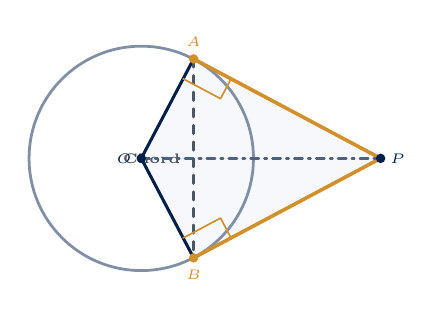
\begin{tikzpicture}[scale=0.95, line cap=round, line join=round]
  \coordinate (O) at (0,0);
  \def\r{1.5}
  \def\d{3.2}
  \coordinate (P) at (\d,0);
  \coordinate (A) at (0.7, 1.33);
  \coordinate (B) at (0.7, -1.33);

  \fill[bluepale!60] (O) -- (A) -- (P) -- (B) -- cycle;
  \draw[navy!50, line width=1pt] (O) circle (\r);

  \draw[accent, line width=1.3pt] (P) -- (A);
  \draw[accent, line width=1.3pt] (P) -- (B);
  \draw[navy, line width=1.1pt] (O) -- (A);
  \draw[navy, line width=1.1pt] (O) -- (B);
  \draw[secondary, line width=1pt, dashed] (A) -- (B) node[midway, left=1pt, font=\tiny\bfseries\color{secondary}]{Chord};
  \draw[navy!70, line width=0.9pt, dashdotted] (O) -- (P);

  \draw[accent, line width=0.6pt] ($(A)!0.2!(P)$) -- ($(A)!0.2!(P) + (A)!0.2!(O) - (A)$) -- ($(A)!0.2!(O)$);
  \draw[accent, line width=0.6pt] ($(B)!0.2!(P)$) -- ($(B)!0.2!(P) + (B)!0.2!(O) - (B)$) -- ($(B)!0.2!(O)$);

  \fill[navy] (O) circle (1.8pt) node[left, font=\tiny\bfseries\color{navy}]{$O$};
  \fill[primary] (P) circle (1.8pt) node[right, font=\tiny\bfseries\color{primary}]{$P$};
  \fill[accent] (A) circle (1.8pt) node[above=1pt, font=\tiny\bfseries\color{accent}]{$A$};
  \fill[accent] (B) circle (1.8pt) node[below=1pt, font=\tiny\bfseries\color{accent}]{$B$};
\end{tikzpicture}
\end{center}

\vspace{-2mm}
\begin{formulaBox}
  \textbf{The Supplementary Tangent-Angle Theorem:} \\
  The angle between two tangents is supplementary to the angle subtended by contact points at centre:
  \[
    \boxed{\angle APB + \angle AOB = 180^\circ}
  \]
  \textit{Proof:} In quadrilateral $OAPB$: $\angle OAP + \angle AOB + \angle OBP + \angle APB = 360^\circ$. \\
  Since $\angle OAP = \angle OBP = 90^\circ$: $90^\circ + \angle AOB + 90^\circ + \angle APB = 360^\circ \implies \mathbf{\angle AOB + \angle APB = 180^\circ}$. \\
  \textbf{Deduction:} Quadrilateral $OAPB$ is a \textbf{cyclic quadrilateral}.
\end{formulaBox}

\subhead{Module 6.2 $\vert$ Angle with Chord of Contact ($AB$)}

Since $PA = PB$, $\triangle PAB$ is an \textbf{isosceles triangle}:
\begin{enumerate}[itemsep=1.5pt]
  \item $\angle PAB = \angle PBA = \frac{180^\circ - \angle APB}{2} = 90^\circ - \frac{1}{2}\angle APB$.
  \item Since $\angle OAP = 90^\circ$, we have $\angle OAB = 90^\circ - \angle PAB = \frac{1}{2}\angle APB$.
  \item Hence:
    \[
      \boxed{\angle APB = 2\angle OAB}
    \]
\end{enumerate}

\subhead{Module 6.3 $\vert$ Worked Board Archetype}

\begin{conceptBox}[title=Worked Archetype 3: Tangents Inclined at $60^\circ$,fonttitle=\bfseries\color{navy}]
  \textbf{Problem:} Two tangents $PA, PB$ have $\angle APB = 60^\circ$. If $OP = 10\text{ cm}$, find radius $r$ and tangent length.\\
  \textbf{Solution:}
  \begin{enumerate}[leftmargin=5mm, itemsep=1pt]
    \item $OP$ bisects $\angle APB$, so $\angle OPA = 30^\circ$. In right $\triangle OAP$ ($\angle OAP = 90^\circ$):
    \item $\sin 30^\circ = \frac{r}{OP} \implies \frac{1}{2} = \frac{r}{10} \implies \mathbf{r = 5\text{ cm}}$.
    \item $\cos 30^\circ = \frac{PA}{OP} \implies \frac{\sqrt{3}}{2} = \frac{PA}{10} \implies \mathbf{PA = 5\sqrt{3}\text{ cm}}$.
  \end{enumerate}
\end{conceptBox}

\clearpage

% =============================================================================
% PAGE 8: MODULE 7 — TANGENTS IN POLYGONS (INCIRCLES & QUADRILATERALS)
% =============================================================================
\thispagestyle{fancy}
\vspace*{0mm}

\chapterbanner{10}{TANGENTS IN TRIANGLES \& QUADRILATERALS}{Incircle Splitting, Circumscribed Quadrilateral ($AB+CD=AD+BC$) \& Rhombus}{\CoreTag}

\subhead{Module 7.1 $\vert$ Circle Inscribed in a Triangle (Tangent Splitting)}

When a circle with centre $O$ and radius $r$ is inscribed in $\triangle ABC$, it touches sides $BC, CA, AB$ at $D, E, F$:

\begin{center}
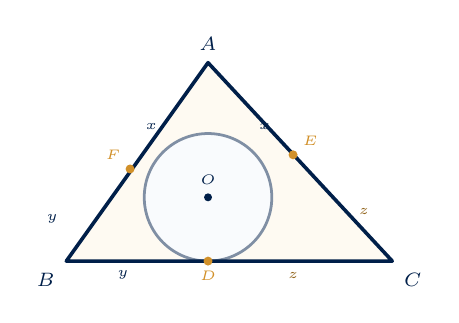
\begin{tikzpicture}[scale=0.9, line cap=round, line join=round]
  \coordinate (A) at (2.0, 2.8);
  \coordinate (B) at (0, 0);
  \coordinate (C) at (4.6, 0);

  % Incircle approximations
  \coordinate (Incenter) at (2.0, 0.9);
  \fill[accentlight] (A) -- (B) -- (C) -- cycle;
  \draw[navy!50, fill=bluepale!40, line width=1pt] (Incenter) circle (0.9);
  \draw[navy, line width=1.3pt] (A) -- (B) -- (C) -- cycle;

  \coordinate (D) at (2.0, 0);
  \coordinate (E) at (3.2, 1.5);
  \coordinate (F) at (0.9, 1.3);

  \fill[accent] (D) circle (1.8pt) node[below, font=\tiny\bfseries\color{accent}]{$D$};
  \fill[accent] (E) circle (1.8pt) node[above right, font=\tiny\bfseries\color{accent}]{$E$};
  \fill[accent] (F) circle (1.8pt) node[above left, font=\tiny\bfseries\color{accent}]{$F$};
  \fill[navy] (Incenter) circle (1.6pt) node[above=1pt, font=\tiny\bfseries\color{navy}]{$O$};

  \node[font=\tiny\bfseries\color{primary}] at (1.2, 1.9) {$x$};
  \node[font=\tiny\bfseries\color{primary}] at (2.8, 1.9) {$x$};
  \node[font=\tiny\bfseries\color{navy}] at (-0.2, 0.6) {$y$};
  \node[font=\tiny\bfseries\color{navy}] at (0.8, -0.2) {$y$};
  \node[font=\tiny\bfseries\color{gold!70!black}] at (3.2, -0.2) {$z$};
  \node[font=\tiny\bfseries\color{gold!70!black}] at (4.2, 0.7) {$z$};

  \node[above=1pt, font=\scriptsize\bfseries\color{navy}] at (A) {$A$};
  \node[below left=1pt, font=\scriptsize\bfseries\color{navy}] at (B) {$B$};
  \node[below right=1pt, font=\scriptsize\bfseries\color{navy}] at (C) {$C$};
\end{tikzpicture}
\end{center}

\vspace{-2mm}
\begin{formulaBox}
  Tangent segments from each vertex are equal: $AF = AE = x$, $BD = BF = y$, $CD = CE = z$.
  \[
    \boxed{AF = x = s - a} \qquad \boxed{BD = y = s - b} \qquad \boxed{CD = z = s - c} \qquad \boxed{\text{Area}(\triangle ABC) = r \cdot s}
  \]
  where $s = \frac{a+b+c}{2}$ is the semi-perimeter.
\end{formulaBox}

\subhead{Module 7.2 $\vert$ Quadrilateral Circumscribing a Circle (The Pitot Theorem)}

\begin{minipage}[t]{0.56\textwidth}
  \textbf{CBSE Classic Theorem:} \\
  \textit{If quadrilateral $ABCD$ circumscribes a circle, then sum of opposite sides are equal:}
  \[
    \boxed{AB + CD = AD + BC}
  \]
  \textbf{Proof:}
  Let the circle touch $AB, BC, CD, DA$ at $P, Q, R, S$.
  \begin{align*}
    AP &= AS \quad \text{--- (1)} & BP &= BQ \quad \text{--- (2)} \\
    CR &= CQ \quad \text{--- (3)} & DR &= DS \quad \text{--- (4)}
  \end{align*}
  Adding (1) + (2) + (3) + (4):
  \[
    (AP + BP) + (CR + DR) = (AS + DS) + (BQ + CQ)
  \]
  \[
    \mathbf{AB + CD = AD + BC}. \quad \text{\textbf{[Hence Proved]}}
  \]
\end{minipage}\hfill
\begin{minipage}[t]{0.41\textwidth}
  \begin{center}
  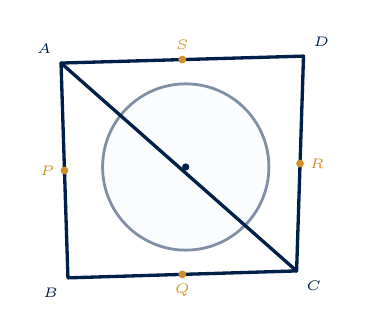
\begin{tikzpicture}[scale=0.88, line cap=round, line join=round]
    \coordinate (O) at (0,0);
    \draw[navy!50, fill=bluepale!30, line width=1pt] (O) circle (1.2);
    \fill[navy] (O) circle (1.5pt);

    \coordinate (A) at (-1.8, 1.5);
    \coordinate (B) at (-1.7, -1.6);
    \coordinate (C) at (1.6, -1.5);
    \coordinate (D) at (1.7, 1.6);

    \draw[navy, line width=1.2pt] (A) -- (B) -- (C) -- cycle;
    \draw[navy, line width=1.2pt] (A) -- (D) -- (C);
    \node[above left, font=\tiny\bfseries\color{navy}] at (A) {$A$};
    \node[below left, font=\tiny\bfseries\color{navy}] at (B) {$B$};
    \node[below right, font=\tiny\bfseries\color{navy}] at (C) {$C$};
    \node[above right, font=\tiny\bfseries\color{navy}] at (D) {$D$};

    \fill[accent] ($(A)!0.5!(B)$) circle (1.6pt) node[left, font=\tiny\bfseries\color{accent}]{$P$};
    \fill[accent] ($(B)!0.5!(C)$) circle (1.6pt) node[below, font=\tiny\bfseries\color{accent}]{$Q$};
    \fill[accent] ($(C)!0.5!(D)$) circle (1.6pt) node[right, font=\tiny\bfseries\color{accent}]{$R$};
    \fill[accent] ($(D)!0.5!(A)$) circle (1.6pt) node[above, font=\tiny\bfseries\color{accent}]{$S$};
  \end{tikzpicture}
  \end{center}
\end{minipage}

\vspace{-1mm}
\begin{successBox}[title=Circumscribed Parallelogram is a Rhombus,fonttitle=\bfseries\color{green}]
  If $ABCD$ is a parallelogram circumscribing a circle:
  $AB = CD$ and $AD = BC$. Then $AB + CD = AD + BC \implies 2AB = 2AD \implies AB = AD$.
  Since adjacent sides are equal, \textbf{$ABCD$ is a Rhombus}.
\end{successBox}

\clearpage

% =============================================================================
% PAGE 9: MODULE 8 — WORKED BOARD-EXAM MASTER MODELS
% =============================================================================
\thispagestyle{fancy}
\vspace*{0mm}

\chapterbanner{10}{WORKED BOARD-EXAM MASTER MODELS}{Concentric Circles, Right-Triangle Incircle \& Chord Geometry}{\WorkedTag}

\subhead{Module 8.1 $\vert$ Model 1: Concentric Circles Chord-Tangent Theorem}

\begin{minipage}[t]{0.56\textwidth}
  \textbf{Problem (CBSE Standard 3-Mark Question):} \\
  \textit{Two concentric circles have radii $5\text{ cm}$ and $3\text{ cm}$. Find the length of the chord of the larger circle which touches the smaller circle.}

  \vspace{1mm}
  \textbf{Solution:}
  \begin{enumerate}[leftmargin=4.5mm, itemsep=1.5pt]
    \item Let $O$ be common centre, $C_1$ ($R=5$) and $C_2$ ($r=3$).
    \item Chord $AB$ of $C_1$ touches $C_2$ at $P$.
    \item By Theorem 10.1, $OP \perp AB$.
    \item Perpendicular from centre to chord bisects the chord: $AP = PB = \frac{1}{2}AB$.
    \item In right $\triangle OPA$:
      \[
        AP = \sqrt{R^2 - r^2} = \sqrt{5^2 - 3^2} = \sqrt{16} = 4\text{ cm}
      \]
    \item $\text{Chord } AB = 2 \times AP = 2 \times 4 = \mathbf{8\text{ cm}}$.
  \end{enumerate}
\end{minipage}\hfill
\begin{minipage}[t]{0.41\textwidth}
  \begin{center}
  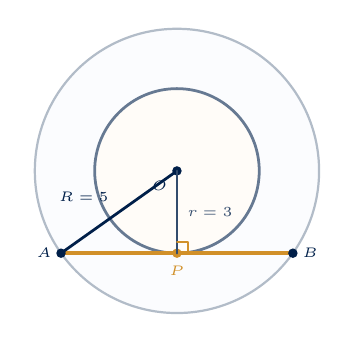
\begin{tikzpicture}[scale=0.95, line cap=round, line join=round]
    \coordinate (O) at (0,0);
    \def\rsmall{1.1}
    \def\rlarge{1.9}

    \draw[navy!30, fill=bluepale!25, line width=0.8pt] (O) circle (\rlarge);
    \draw[navy!60, fill=accentlight!50, line width=1pt] (O) circle (\rsmall);
    \fill[navy] (O) circle (1.8pt) node[below left, font=\tiny\bfseries\color{navy}]{$O$};

    \coordinate (P) at (0, -\rsmall);
    \coordinate (A) at (-1.55, -\rsmall);
    \coordinate (B) at (1.55, -\rsmall);

    \draw[accent, line width=1.3pt] (A) -- (B);
    \fill[primary] (A) circle (1.8pt) node[left, font=\tiny\bfseries\color{primary}]{$A$};
    \fill[primary] (B) circle (1.8pt) node[right, font=\tiny\bfseries\color{primary}]{$B$};
    \fill[accent] (P) circle (1.8pt) node[below=1pt, font=\tiny\bfseries\color{accent}]{$P$};

    \draw[navy, line width=1pt] (O) -- (A) node[midway, above left, font=\tiny\bfseries]{$R=5$};
    \draw[primary!80, line width=1pt] (O) -- (P) node[midway, right, font=\tiny\bfseries]{$r=3$};
    \draw[accent, line width=0.6pt] (0.15,-\rsmall) -- (0.15,-\rsmall+0.15) -- (0,-\rsmall+0.15);
  \end{tikzpicture}
  \end{center}
\end{minipage}

\begin{formulaBox}
  \textbf{General Concentric Chord Formula:} \quad $\boxed{\text{Length of chord } AB = 2\sqrt{R^2 - r^2}}$
\end{formulaBox}

\subhead{Module 8.2 $\vert$ Model 2: Incircle of a Right-Angled Triangle}

\begin{minipage}[t]{0.56\textwidth}
  \textbf{Problem (High-Frequency Board Archetype):} \\
  A circle is inscribed in right $\triangle ABC$ ($\angle B = 90^\circ$). With sides $a, c$ and hypotenuse $b$, prove inradius:
  \[
    \boxed{r = \frac{a + c - b}{2}}
  \]
  \textbf{Proof:}
  Let the circle touch $BC$ at $D$, $AB$ at $F$, and $AC$ at $E$.
  \begin{itemize}[itemsep=1pt]
    \item Since $OF \perp AB$ and $OD \perp BC$, $OFBD$ has three $90^\circ$ angles and adjacent sides equal ($OF=OD=r$). Thus, \textbf{$OFBD$ is a square}.
    \item Hence, $BF = BD = r$.
    \item $AE = AF = c - r$ and $CE = CD = a - r$.
    \item Hypotenuse $b = AE + CE = (c - r) + (a - r) = a + c - 2r$.
    \item Rearranging: $2r = a + c - b \implies \mathbf{r = \frac{a + c - b}{2}}$.
  \end{itemize}
\end{minipage}\hfill
\begin{minipage}[t]{0.41\textwidth}
  \begin{center}
  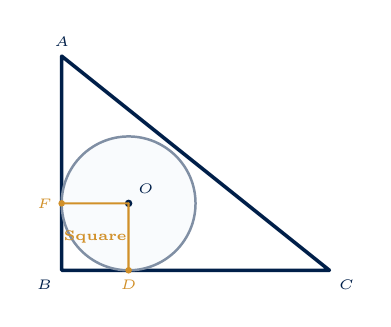
\begin{tikzpicture}[scale=0.85, line cap=round, line join=round]
    \coordinate (B) at (0,0);
    \coordinate (A) at (0,3.2);
    \coordinate (C) at (4.0,0);

    \draw[navy, line width=1.3pt] (A) -- (B) -- (C) -- cycle;
    \node[above, font=\tiny\bfseries\color{navy}] at (A) {$A$};
    \node[below left, font=\tiny\bfseries\color{navy}] at (B) {$B$};
    \node[below right, font=\tiny\bfseries\color{navy}] at (C) {$C$};

    \coordinate (O) at (1.0, 1.0);
    \draw[navy!50, fill=bluepale!40, line width=0.9pt] (O) circle (1.0);
    \fill[navy] (O) circle (1.6pt) node[above right, font=\tiny\bfseries]{$O$};

    \draw[accent, line width=0.8pt] (O) -- (1.0,0);
    \draw[accent, line width=0.8pt] (O) -- (0,1.0);
    \fill[accent] (1.0,0) circle (1.4pt) node[below, font=\tiny\bfseries]{$D$};
    \fill[accent] (0,1.0) circle (1.4pt) node[left, font=\tiny\bfseries]{$F$};

    \node[font=\tiny\bfseries\color{accent}] at (0.5, 0.5) {Square};
  \end{tikzpicture}
  \end{center}
\end{minipage}

\clearpage

% =============================================================================
% PAGE 10: MODULE 9 — COMMON TANGENTS TO TWO CIRCLES
% =============================================================================
\thispagestyle{fancy}
\vspace*{0mm}

\chapterbanner{10}{COMMON TANGENTS TO TWO CIRCLES}{Relative Positions, Centre Distances \& Tangent Counts}{\ExtensionTag}

\subhead{Module 9.1 $\vert$ Direct vs. Transverse Common Tangents}
A \textbf{common tangent} touches both circles simultaneously:
\begin{itemize}
  \item \textbf{Direct (External):} Both circles lie on the \textbf{same side} of the tangent line.
  \item \textbf{Transverse (Internal):} Circles lie on \textbf{opposite sides} of the tangent (line crosses centre segment).
\end{itemize}

\subhead{Module 9.2 $\vert$ The Five Positional Configurations}
Let two circles have radii $r_1, r_2$ ($r_1 \ge r_2$) and centre-to-centre distance $d = O_1O_2$:

\begin{center}
\small
\begin{tabularx}{\textwidth}{c >{\bfseries\color{navy}}p{26mm} c c X}
\toprule
\rowcolor{bluepale}Case & Configuration & Condition on $d$ & Total & Breakdown \\
\midrule
1 & Disjoint (Separate) & $d > r_1 + r_2$ & \textbf{4} & $2 \text{ Direct} + 2 \text{ Transverse}$ \\
2 & Touching Externally & $d = r_1 + r_2$ & \textbf{3} & $2 \text{ Direct} + 1 \text{ Transverse}$ \\
3 & Intersecting & $|r_1 - r_2| < d < r_1 + r_2$ & \textbf{2} & $2 \text{ Direct} + 0 \text{ Transverse}$ \\
4 & Touching Internally & $d = r_1 - r_2$ & \textbf{1} & $1 \text{ Direct}$ \\
5 & Concentric / Inside & $d < r_1 - r_2$ & \textbf{0} & No common tangent \\
\bottomrule
\end{tabularx}
\end{center}

\vspace{-1mm}
\subhead{Module 9.3 $\vert$ Visual Representations of Common Tangents}

\begin{center}
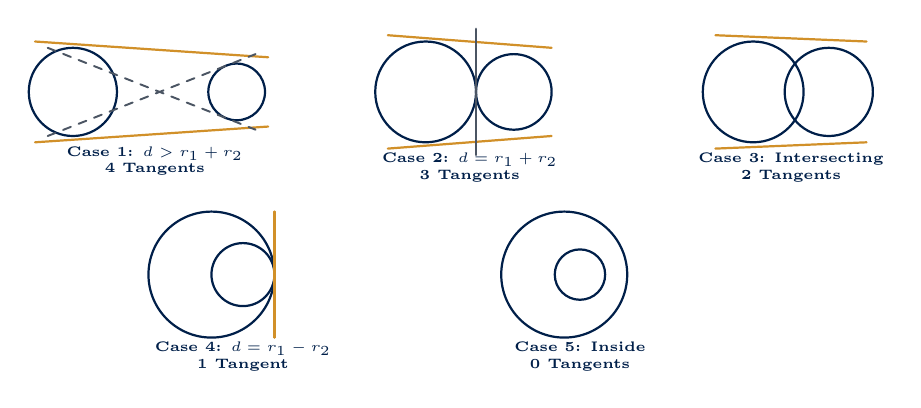
\begin{tikzpicture}[scale=0.8, line cap=round, line join=round]
  % Case 1
  \begin{scope}[shift={(0,2.5)}]
    \draw[navy, line width=0.8pt] (0,0) circle (0.7);
    \draw[navy, line width=0.8pt] (2.6,0) circle (0.45);
    \draw[accent, line width=0.8pt] (-0.6, 0.8) -- (3.1, 0.55);
    \draw[accent, line width=0.8pt] (-0.6, -0.8) -- (3.1, -0.55);
    \draw[secondary, line width=0.7pt, dashed] (-0.4, -0.7) -- (2.9, 0.6);
    \draw[secondary, line width=0.7pt, dashed] (-0.4, 0.7) -- (2.9, -0.6);
    \node[font=\tiny\bfseries\color{navy}, align=center] at (1.3,-1.1) {Case 1: $d > r_1+r_2$\\\textbf{4 Tangents}};
  \end{scope}

  % Case 2
  \begin{scope}[shift={(5.6,2.5)}]
    \draw[navy, line width=0.8pt] (0,0) circle (0.8);
    \draw[navy, line width=0.8pt] (1.4,0) circle (0.6);
    \draw[accent, line width=0.8pt] (-0.6, 0.9) -- (2.0, 0.7);
    \draw[accent, line width=0.8pt] (-0.6, -0.9) -- (2.0, -0.7);
    \draw[secondary, line width=0.9pt] (0.8, -1.0) -- (0.8, 1.0);
    \node[font=\tiny\bfseries\color{navy}, align=center] at (0.7,-1.2) {Case 2: $d = r_1+r_2$\\\textbf{3 Tangents}};
  \end{scope}

  % Case 3
  \begin{scope}[shift={(10.8,2.5)}]
    \draw[navy, line width=0.8pt] (0,0) circle (0.8);
    \draw[navy, line width=0.8pt] (1.2,0) circle (0.7);
    \draw[accent, line width=0.8pt] (-0.6, 0.9) -- (1.8, 0.8);
    \draw[accent, line width=0.8pt] (-0.6, -0.9) -- (1.8, -0.8);
    \node[font=\tiny\bfseries\color{navy}, align=center] at (0.6,-1.2) {Case 3: Intersecting\\\textbf{2 Tangents}};
  \end{scope}

  % Case 4
  \begin{scope}[shift={(2.2,-0.4)}]
    \draw[navy, line width=0.8pt] (0,0) circle (1.0);
    \draw[navy, line width=0.8pt] (0.5,0) circle (0.5);
    \draw[accent, line width=0.9pt] (1.0, -1.0) -- (1.0, 1.0);
    \node[font=\tiny\bfseries\color{navy}, align=center] at (0.5,-1.3) {Case 4: $d = r_1-r_2$\\\textbf{1 Tangent}};
  \end{scope}

  % Case 5
  \begin{scope}[shift={(7.8,-0.4)}]
    \draw[navy, line width=0.8pt] (0,0) circle (1.0);
    \draw[navy, line width=0.8pt] (0.25,0) circle (0.4);
    \node[font=\tiny\bfseries\color{navy}, align=center] at (0.25,-1.3) {Case 5: Inside\\\textbf{0 Tangents}};
  \end{scope}
\end{tikzpicture}
\end{center}

\vspace{-1mm}
\begin{warningBox}[title=Enrichment / Extension Scope Note,fonttitle=\bfseries\color{navy}]
  The classification of common tangents is an \textbf{extension topic} useful for conceptual clarity and 1-mark objective questions. Length calculations of common tangents are strictly non-evaluative for Class 10 board exams.
\end{warningBox}

\clearpage

% =============================================================================
% PAGE 11: MODULE 10 — MASTER SUMMARY & QUICK-REFERENCE MATRIX
% =============================================================================
\thispagestyle{fancy}
\vspace*{0mm}

\chapterbanner{10}{MASTER SUMMARY \& FORMULA MATRIX}{The Complete Geometric Reference Sheet for Board Quick-Revision}{\ReferenceTag}

\subhead{Module 10.1 $\vert$ Comprehensive Theorem \& Formula Repository}

\begin{center}
\small
\begin{tabularx}{\textwidth}{>{\bfseries\color{navy}}p{30mm} >{\bfseries\color{primary}}p{40mm} X}
\toprule
\rowcolor{bluepale}Concept / Theorem & Core Formula / Statement & Key Geometric Implication \\
\midrule
Theorem 10.1 & $OP \perp \text{Tangent at } P$ & Radius to point of contact makes $90^\circ$. Right triangle for Pythagoras. \\
Theorem 10.2 & $PA = PB$ & Tangents from external point are equal in length. Forms isosceles $\triangle PAB$. \\
OP as Angle Bisector & $\angle OPA = \angle OPB = \frac{1}{2}\angle APB$ & Line of centres bisects angle between tangents and central angle. \\
Supplementary Angles & $\angle AOB + \angle APB = 180^\circ$ & Quadrilateral $OAPB$ is cyclic. $\angle \text{centre} + \angle \text{external} = 180^\circ$. \\
Angle with Chord & $\angle OAB = \frac{1}{2}\angle APB$ & Angle between radius and chord is half the angle between tangents. \\
Pythagoras Relation & $PT = \sqrt{OP^2 - r^2}$ & Directly computes tangent length given distance from centre and radius. \\
Circumscribed Quad & $AB + CD = AD + BC$ & Sum of opposite sides of circumscribed quadrilateral are equal. \\
Circumscribed $\|gm$ & $ABCD \text{ is a Rhombus}$ & A circumscribed parallelogram has all 4 sides equal. \\
Concentric Chord & $\text{Chord } = 2\sqrt{R^2 - r^2}$ & Chord of larger circle touching smaller circle is bisected at contact. \\
Right Triangle Incircle & $r = \frac{a + c - b}{2}$ & Rapid formula for inradius given legs $a, c$ and hypotenuse $b$. \\
General Triangle Incircle & $\Delta = r \cdot s \implies r = \frac{\Delta}{s}$ & Connects triangle area, inradius, and semi-perimeter. \\
\bottomrule
\end{tabularx}
\end{center}

\vspace{-1mm}
\subhead{Module 10.2 $\vert$ Visual Concept Map: Unified Symmetries Blueprint}

\begin{center}
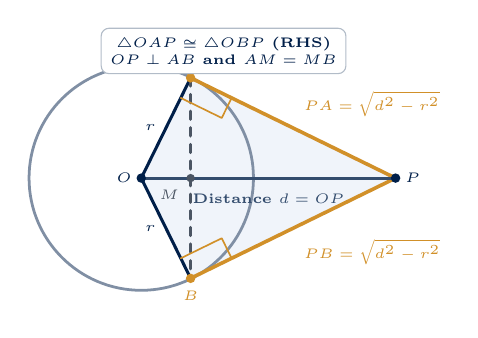
\begin{tikzpicture}[scale=0.95, line cap=round, line join=round]
  \coordinate (O) at (0,0);
  \def\r{1.5}
  \def\d{3.4}
  \coordinate (P) at (\d, 0);
  \coordinate (A) at (0.66, 1.34);
  \coordinate (B) at (0.66, -1.34);
  \coordinate (M) at (0.66, 0);

  \fill[bluepale] (O) -- (A) -- (P) -- (B) -- cycle;
  \draw[navy!50, line width=1pt] (O) circle (\r);

  \draw[accent, line width=1.3pt] (P) -- (A) node[midway, above right, font=\tiny\bfseries\color{accent}]{$PA = \sqrt{d^2-r^2}$};
  \draw[accent, line width=1.3pt] (P) -- (B) node[midway, below right, font=\tiny\bfseries\color{accent}]{$PB = \sqrt{d^2-r^2}$};

  \draw[navy, line width=1.1pt] (O) -- (A) node[midway, left, font=\tiny\bfseries]{$r$};
  \draw[navy, line width=1.1pt] (O) -- (B) node[midway, left, font=\tiny\bfseries]{$r$};
  \draw[navy!80, line width=1.1pt] (O) -- (P) node[midway, below=2pt, font=\tiny\bfseries\color{navy}]{Distance $d = OP$};
  \draw[secondary, line width=1.1pt, dashed] (A) -- (B);

  \draw[accent, line width=0.6pt] ($(A)!0.2!(P)$) -- ($(A)!0.2!(P) + (A)!0.2!(O) - (A)$) -- ($(A)!0.2!(O)$);
  \draw[accent, line width=0.6pt] ($(B)!0.2!(P)$) -- ($(B)!0.2!(P) + (B)!0.2!(O) - (B)$) -- ($(B)!0.2!(O)$);

  \fill[navy] (O) circle (1.8pt) node[left, font=\tiny\bfseries\color{navy}]{$O$};
  \fill[primary] (P) circle (1.8pt) node[right, font=\tiny\bfseries\color{primary}]{$P$};
  \fill[accent] (A) circle (1.8pt) node[above=1pt, font=\tiny\bfseries\color{accent}]{$A$};
  \fill[accent] (B) circle (1.8pt) node[below=1pt, font=\tiny\bfseries\color{accent}]{$B$};
  \fill[secondary] (M) circle (1.6pt) node[below left=1pt, font=\tiny\bfseries\color{secondary}]{$M$};

  \node[draw=navy!30, fill=white, rounded corners=1mm, font=\tiny\bfseries\color{navy}, align=center] at (1.1, 1.7) {
    $\triangle OAP \cong \triangle OBP$ (RHS)\\
    $OP \perp AB$ and $AM = MB$
  };
\end{tikzpicture}
\end{center}

\clearpage

% =============================================================================
% PAGE 12: BOARD EXAM TRAPS, VERIFICATION HACKS & PRE-SUBMISSION AUDIT
% =============================================================================
\thispagestyle{fancy}
\vspace*{0mm}

\chapterbanner{10}{EXAM TRAPS, HACKS \& PRE-SUBMISSION AUDIT}{Crucial Board Pitfalls, Instant Verification Checks \& Final Protocol}{\TrapTag}

\subhead{Module 11.1 $\vert$ Top 8 CBSE Board Exam Traps in Circles}

\begin{enumerate}[label=\textbf{\color{navy}\arabic*.}, leftmargin=6.5mm, itemsep=2pt]
  \item \textbf{Assuming Hypotenuse is the Tangent:} In $\triangle OTP$, hypotenuse is ALWAYS $OP$ (centre to external point), NOT tangent $PT$. Write $OP^2 = r^2 + PT^2$, never $PT^2 = OP^2 + r^2$.
  \item \textbf{Missing Right-Angle Justification in Proofs:} Whenever setting $\angle OAP = 90^\circ$, you MUST cite: \textit{"Radius is perpendicular to the tangent at point of contact (Theorem 10.1)"}.
  \item \textbf{Incorrect Congruence Criterion for Theorem 10.2:} Do not cite SAS or SSS. The standard NCERT proof strictly uses \textbf{RHS} ($\angle OAP = \angle OBP = 90^\circ$, hypotenuse $OP = OP$, radius $OA = OB = r$).
  \item \textbf{Confusing Central Angle with Arc Angles:} The external tangent angle ($\angle APB$) is supplementary to the central angle ($\angle AOB$), NOT to an inscribed angle on the circumference.
  \item \textbf{Misordering Segments in Circumscribed Quadrilaterals:} When adding equations $AP = AS, BP = BQ, CR = CQ, DR = DS$, ensure left sides form $AB + CD$ and right sides form $AD + BC$.
  \item \textbf{Forgetting Chord Bisection by Perpendicular:} In concentric circles, $OP \perp AB$ bisects chord ($AP = PB$). Don't forget the factor of 2: report $AB = 8\text{ cm}$, not $AP = 4\text{ cm}$.
  \item \textbf{Unit Inconsistency:} Always convert radius and external distance into the same unit ($\text{cm}$) before applying Pythagoras.
  \item \textbf{Assuming Circumscribed Quadrilateral is a Rhombus:} A general circumscribed quadrilateral only satisfies $AB + CD = AD + BC$. It is a rhombus ONLY IF already given to be a parallelogram.
\end{enumerate}

\subhead{Module 11.2 $\vert$ Arithmetic \& Algebraic Verification Hacks}
\begin{itemize}[itemsep=1.5pt]
  \item \textbf{The Hypotenuse Benchmark:} Tangent length $PT$ must strictly be \textbf{less than} distance $OP$ ($PT < OP$).
  \item \textbf{The $180^\circ$ Sanity Check:} Always verify $\angle APB + \angle AOB = 180^\circ$. (e.g. $70^\circ + 110^\circ = 180^\circ$).
  \item \textbf{Right Triangle Inradius Quick Check:} Check $r = \frac{a+c-b}{2}$. For $(6, 8, 10)$: $r = \frac{6+8-10}{2} = 2\text{ cm}$.
\end{itemize}

\subhead{Module 11.3 $\vert$ The 5-Point Pre-Submission Board Exam Audit}

\begin{center}
\small
\begin{tabularx}{\textwidth}{>{\bfseries\color{navy}}c p{44mm} X}
\toprule
\rowcolor{bluepale}Check & Verification Item & Board Evaluation Standard \\
\midrule
$\square$ 1 & Right-Angle Marks in Diagrams & Did you mark right-angle squares at every point of contact ($A, B, T$)? \\
$\square$ 2 & Formal Theorem Citations & Are "Theorem 10.1" and "Theorem 10.2" stated with full geometric reasons? \\
$\square$ 3 & Congruence State \& Reason & Is RHS congruence explicitly stated with 3 criteria (Right angle, Hypotenuse, Radius)? \\
$\square$ 4 & Doubling Concentric Chords & Did you multiply the half-chord by $2$ to give the full chord length $AB$? \\
$\square$ 5 & Final Units Explicitly Stated & Are units ($\text{cm}, \text{m}$) explicitly written after every numerical answer? \\
\bottomrule
\end{tabularx}
\end{center}

\vfill
\begin{center}
  {\color{gold}\rule{0.65\textwidth}{1.2pt}}\par\vspace{2mm}
  {\Large\bfseries\color{navy}Master the Theorems. Construct the Logic. Secure the 100\%.}\par\vspace{1.5mm}
  {\small\bfseries\color{gold}MATHS MANTHAN TUITION CLASSES}\par
  {\footnotesize\color{muted}contact@mathsmanthan.co.in \quad\textbar\quad +91-8171546558 \quad\textbar\quad \url{https://mathsmanthan.co.in}}
\end{center}

\end{document}
